\documentclass[aspectratio=169]{beamer}
\usetheme{Bruno}

\title{Support Diohine agro-pastoralists in their governance of \textit{Faidherbia Albida} trees.}
\author{
    \vspace{-1em}
    L. Broutin$^{a,b,d}$, A. Fallot$^{a,b}$, A. Perrotton$^{c,d}$,\\
    A. Gonin$^{e}$, D. Masse$^{f}$, \textbf{E. Delay}$^{a,g}$
}
\institute{
    \vspace{-1.5em}
    $^{a}$ CIRAD, UMR SENS, F-34398 Montpellier, France

    $^{b}$ SENS, CIRAD, IRD, Paul Valéry Montpellier 3 University, Montpellier, France. 

    $^{c}$ CIRAD, Forêts et Sociétés, F-34398 Montpellier, France.

    $^{d}$ Forêts et Sociétés, Univ Montpellier, CIRAD, Montpellier, France. 

    $^{e}$ University Paris Nanterre, LAVUE laboratory, FR 

    $^{f}$ IRD, Eco\&Sols, Abidjan, Ivory Coast

    $^{g}$ UMI UMMSCO, Cheick Anta Diop University, Dakar, Sénégal
}
\date{\today}
\background{background.jpeg}

\begin{document}

\maketitle

\begin{frame}{Study Area}
    \begin{figure}
        \centering
        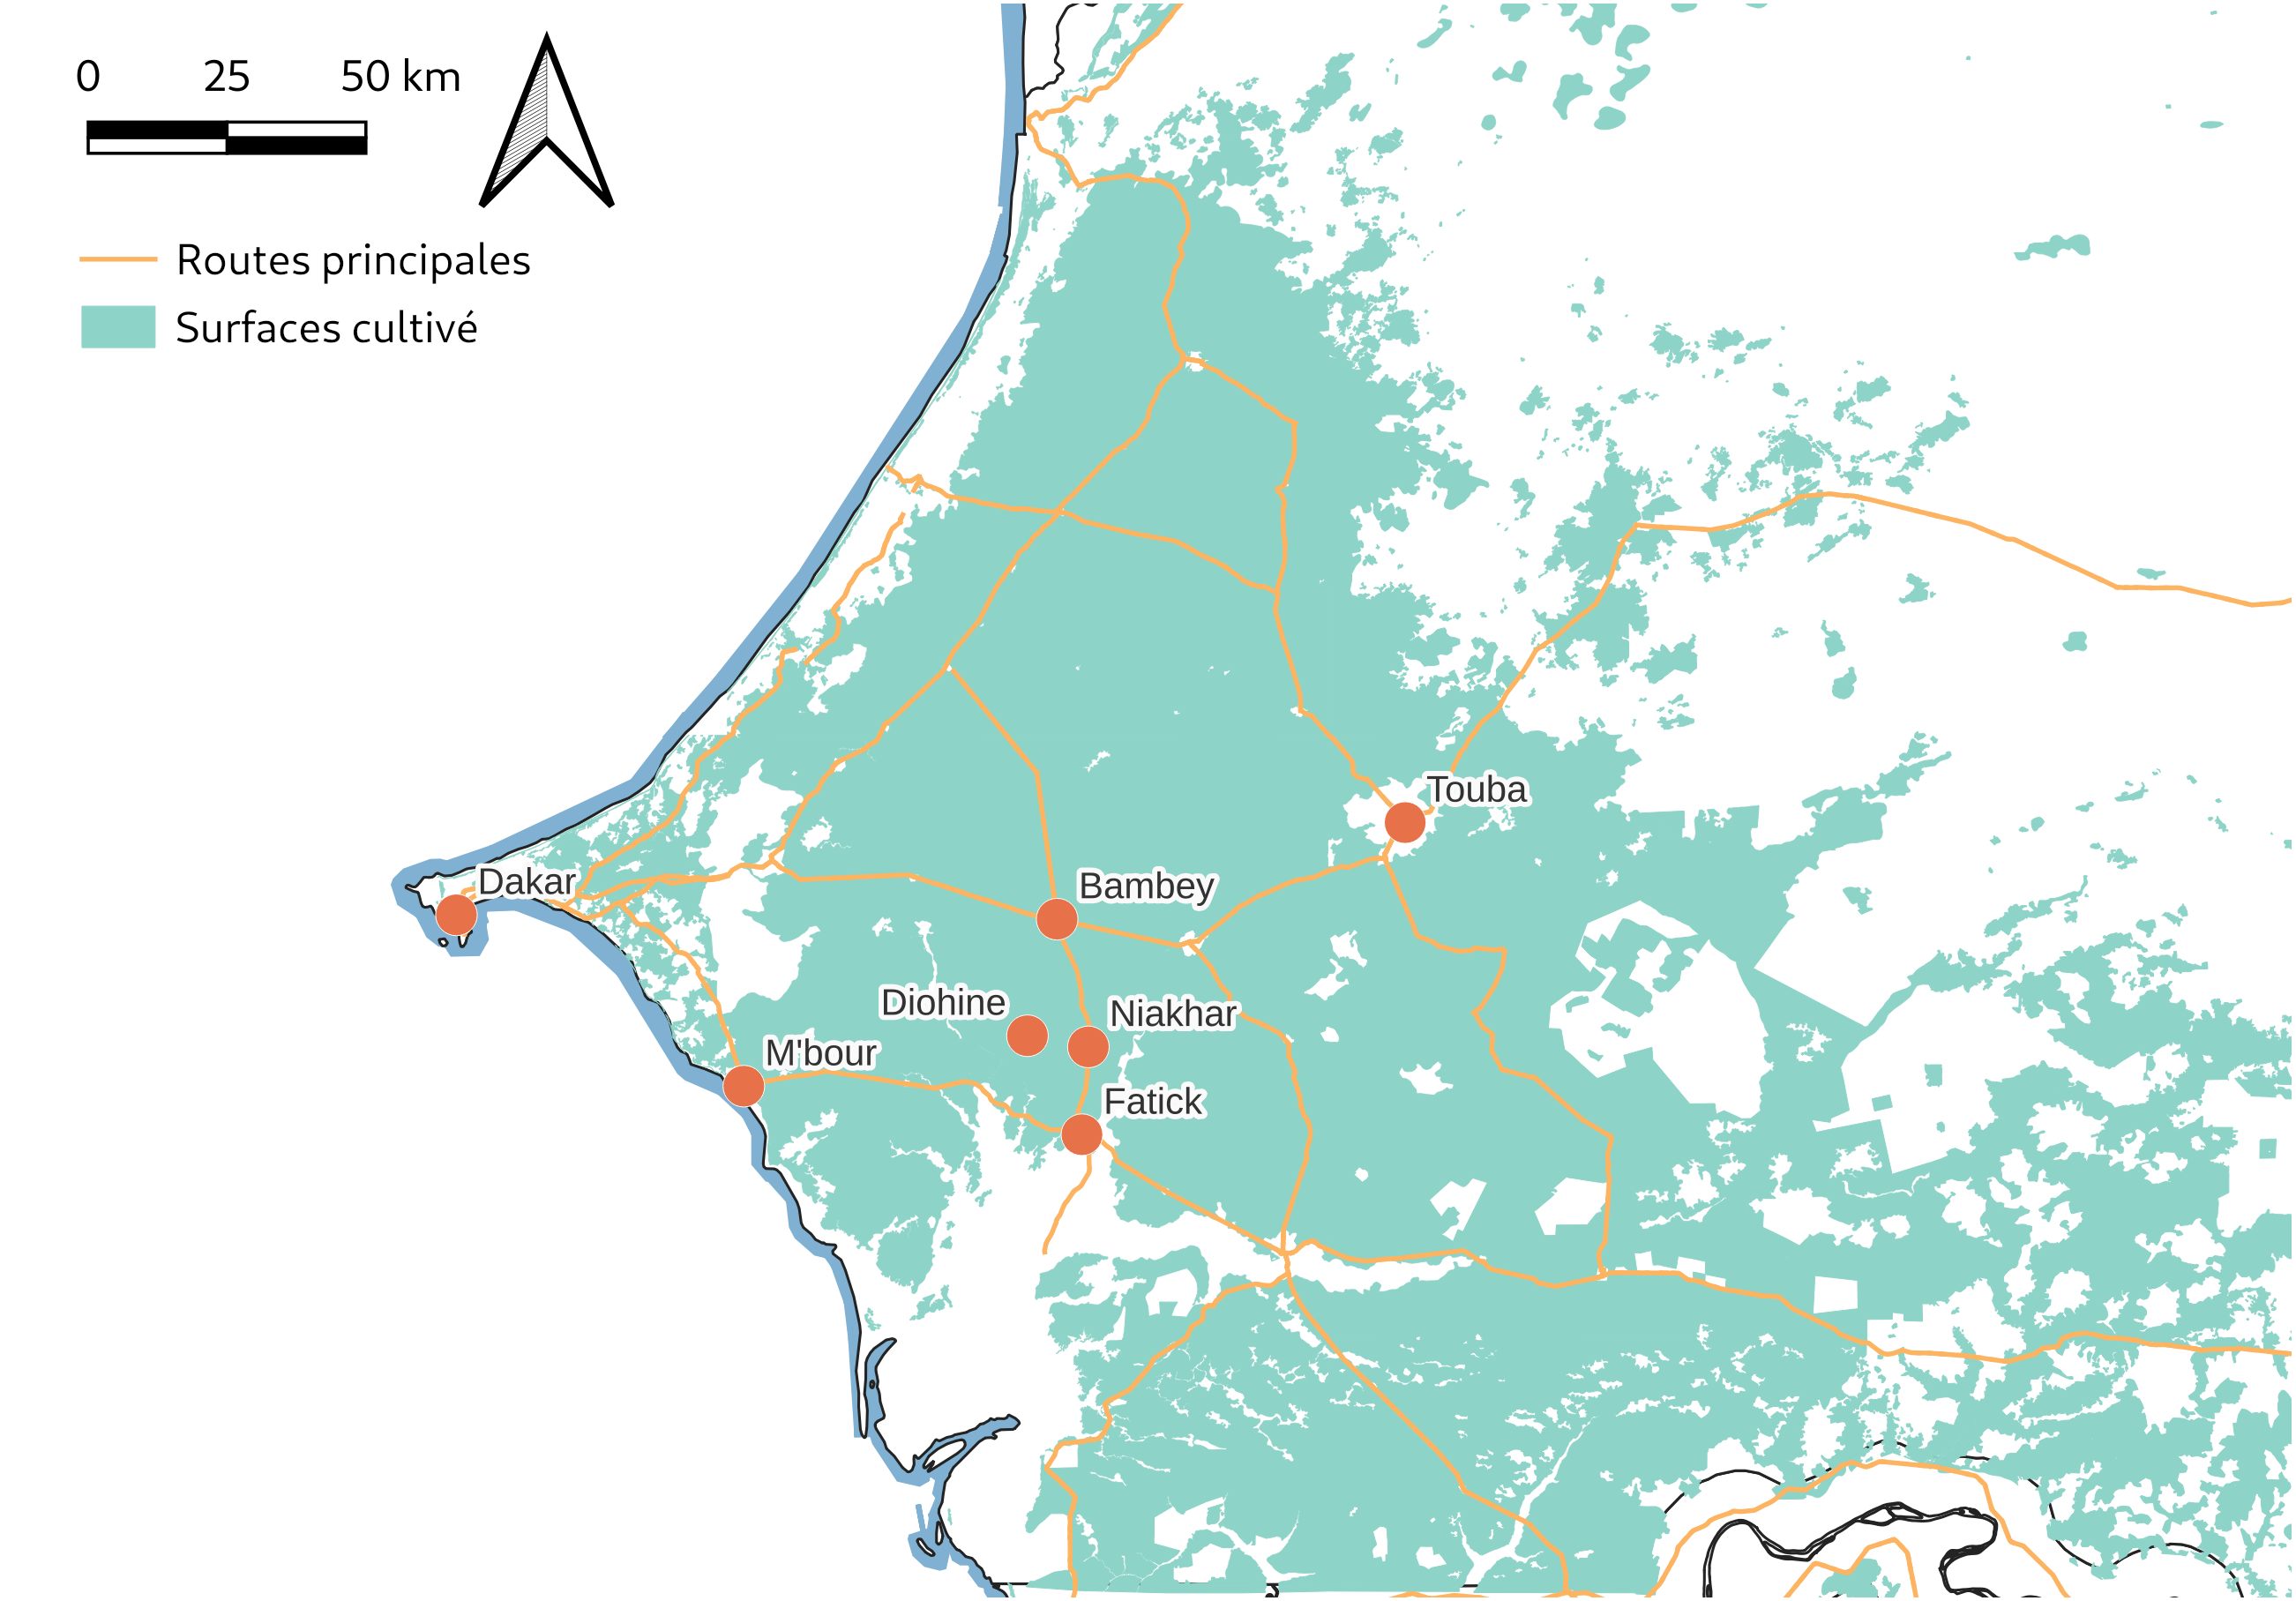
\includegraphics[width=10cm]{img/carte_localisation_diohine.png}
    \end{figure}
\end{frame}

\begin{frame}{Environmental emergency}
    \begin{center}
        \vspace{-1em}
        \begin{figure}
            \centering
            \includegraphics[height = 4.5cm]{img/desert.jpg}~
            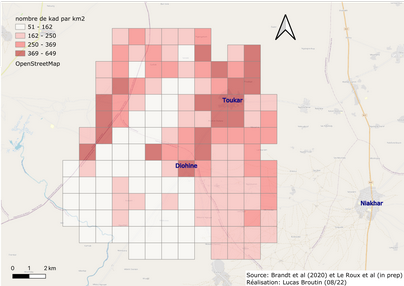
\includegraphics[height = 6cm]{img/densiteArbres.png}
        \end{figure}
    \end{center}
\end{frame}

\begin{frame}{A study rooted in local aspirations : ACADRI}
    \begin{center}
        \vspace{-1em}
        \begin{figure}
            \centering
            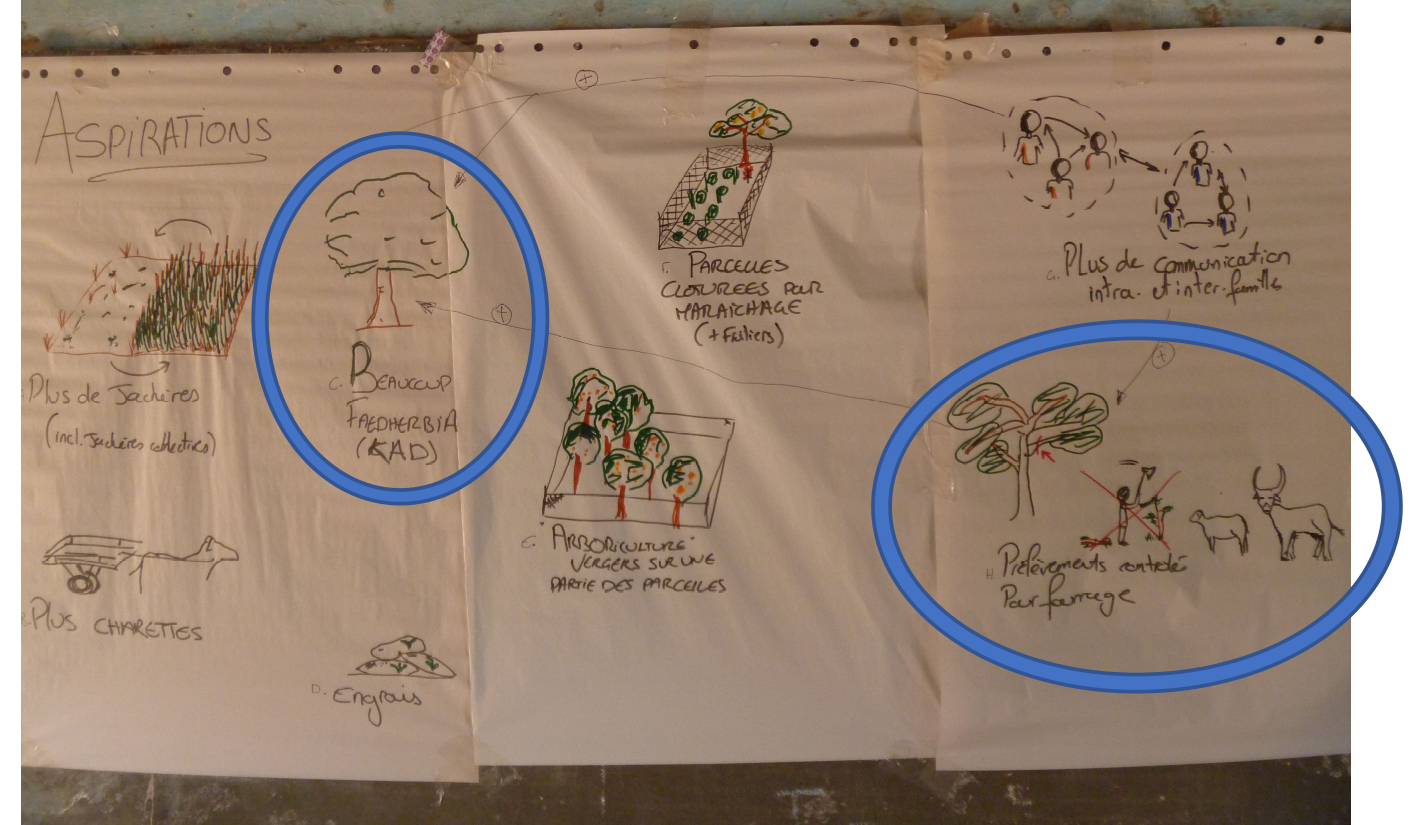
\includegraphics[height = 4.5cm]{img/photoAspiration.png}~
            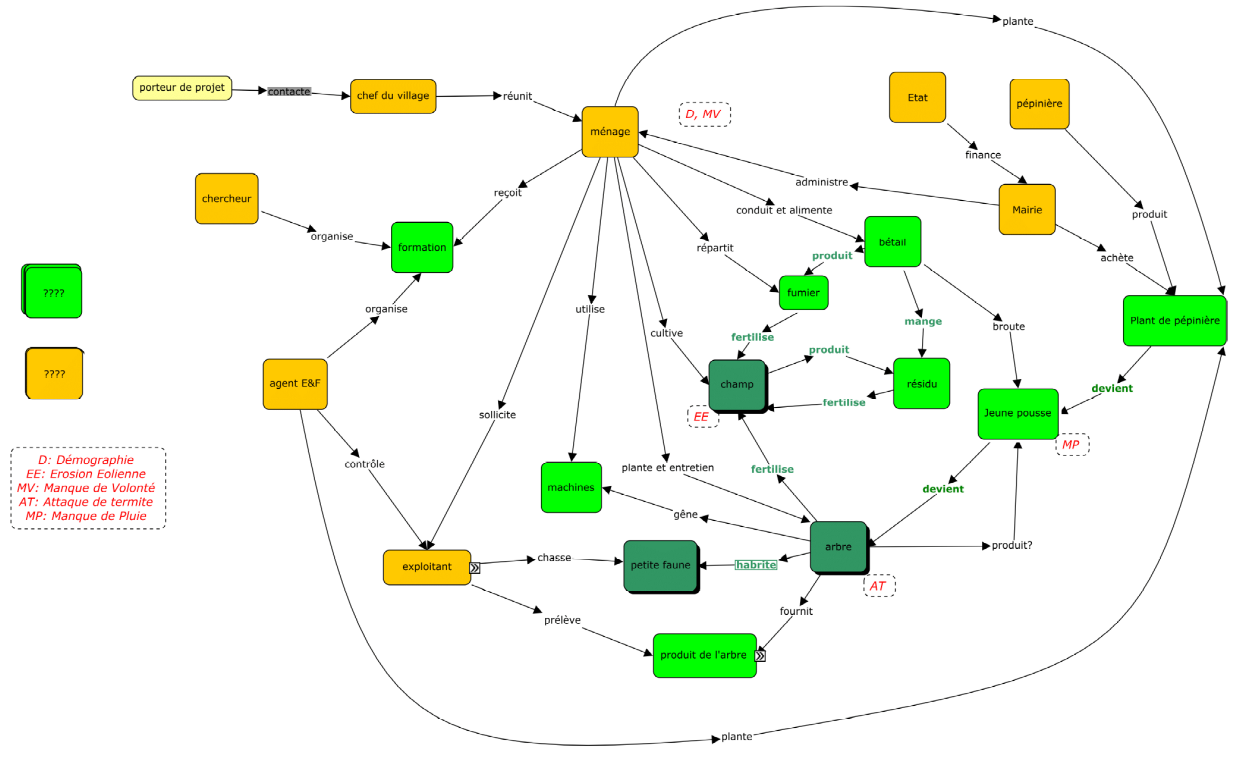
\includegraphics[height = 4.5cm]{img/modeleConceptuel.png}
            \caption{Aspirations expressed during workshop 07/05/2021, Perrotton et al 2021 }
        \end{figure}
    \end{center}
\end{frame}



\begin{frame}{Field issues}
    \begin{center}
        \large{What management of the agroforestry park can be done to deal with environmental degradation ?}
    \end{center}
\end{frame}

\begin{frame}{Field immersion: \\
    Workshops, interviews, participatory approach etc.}
    \begin{center}
        \vspace{-1em}
        \begin{figure}
            \centering
            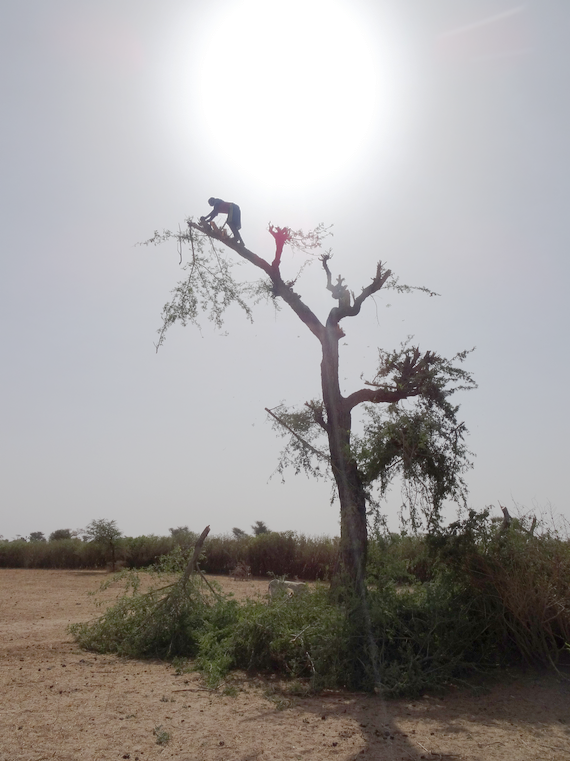
\includegraphics[height = 4.7cm]{img/emondage_faidherbia.png}~
            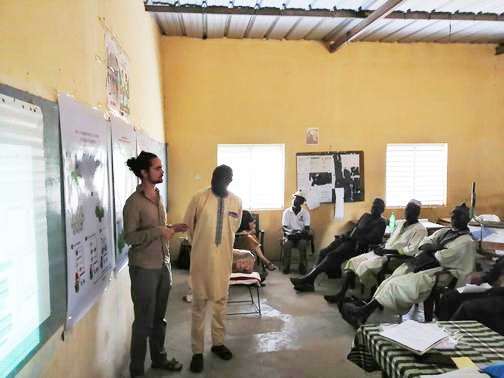
\includegraphics[height = 4.7cm]{img/atelierLucas.jpg}~
            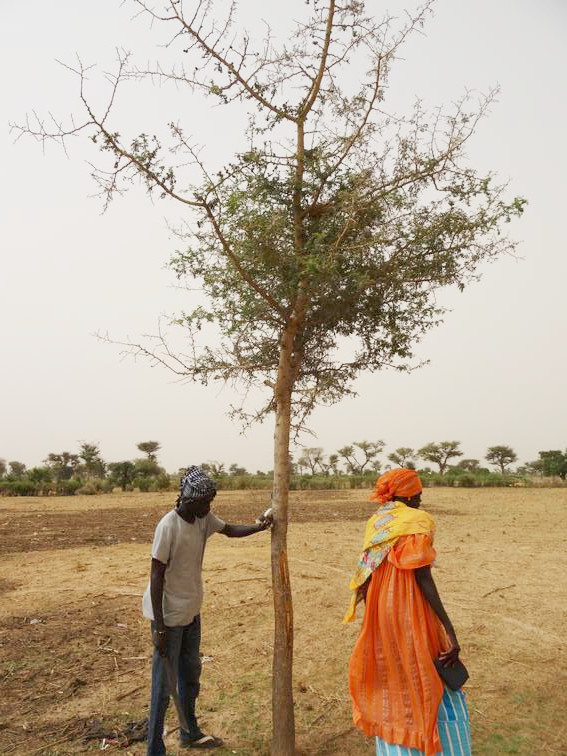
\includegraphics[height = 4.7cm]{img/entretienChamp.jpg}
        \end{figure}
    \end{center}
\end{frame}

\begin{frame}{ComMod : an intelligible model...}
    \begin{center}
        \vspace{-1em}
        \begin{figure}
            \centering
            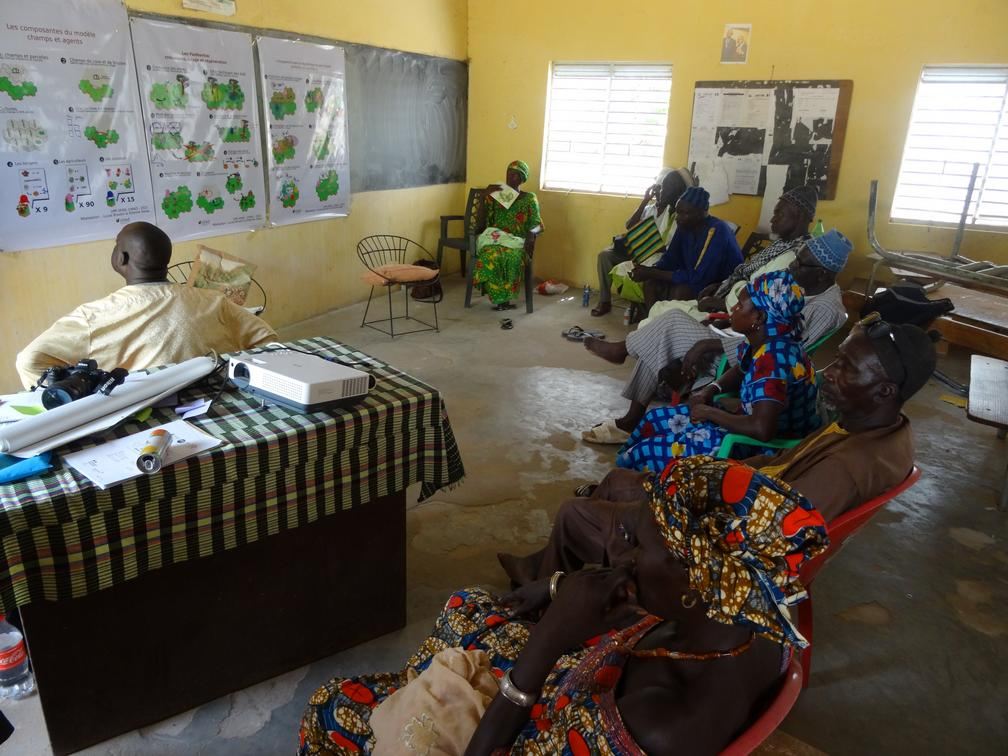
\includegraphics[height = 6cm]{img/atelierPoster.jpg}~
            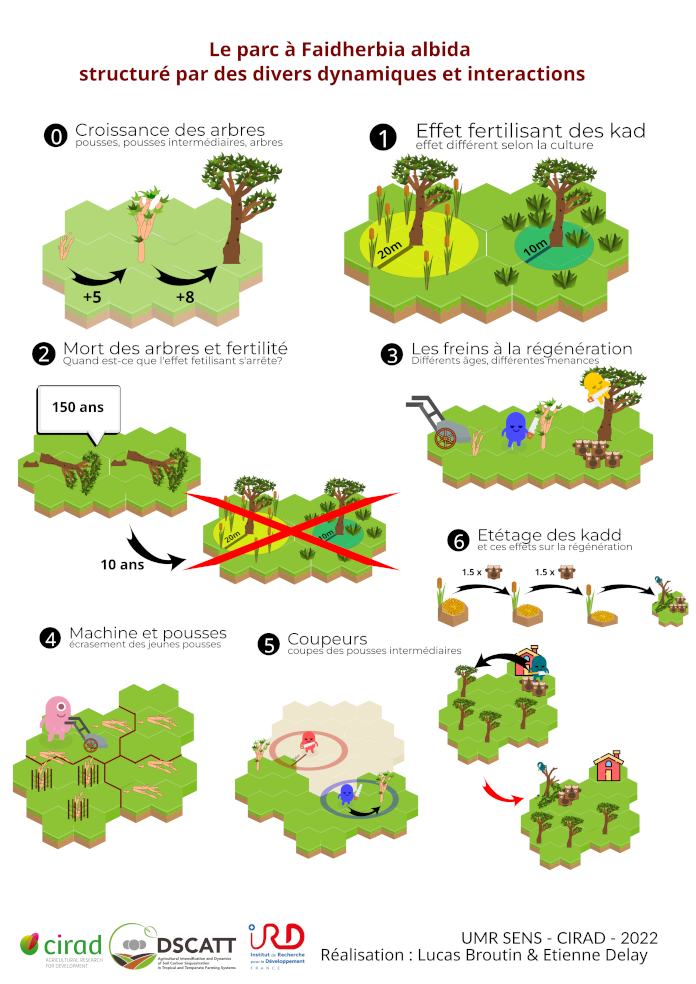
\includegraphics[height = 6cm]{img/poster2.png}
        \end{figure}
    \end{center}
\end{frame}

\begin{frame}{Model as a compass...}
    \begin{itemize}
        \item which guides the "anthropological approach" 
        \item which raises specific questions 
        \item which is based on qualitative data from interviews and workshops  
    \end{itemize}
    \begin{center}
        \vspace{-1em}
        \begin{figure}
            \centering
            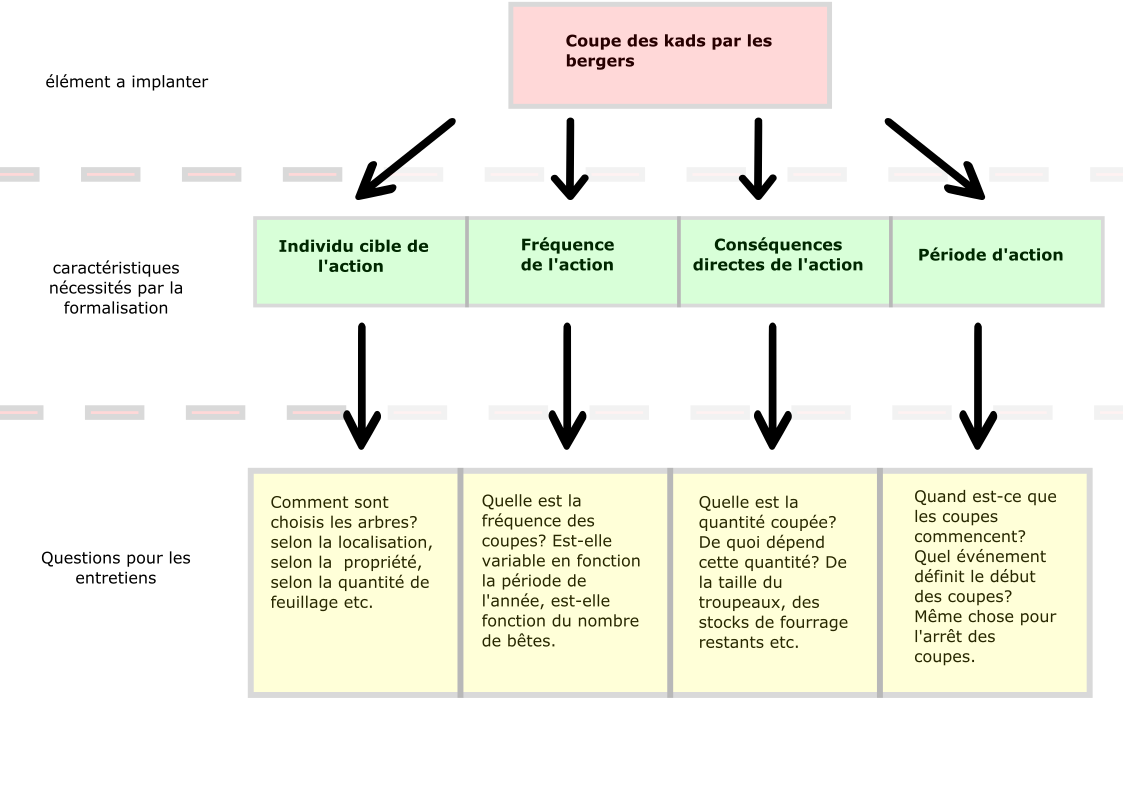
\includegraphics[height = 5.7cm]{img/questionImplementation.png}
        \end{figure}
    \end{center}
\end{frame}

\begin{frame}{... but a model for itself}
    \begin{center}
        \vspace{-1em}
        \begin{figure}
            \centering
            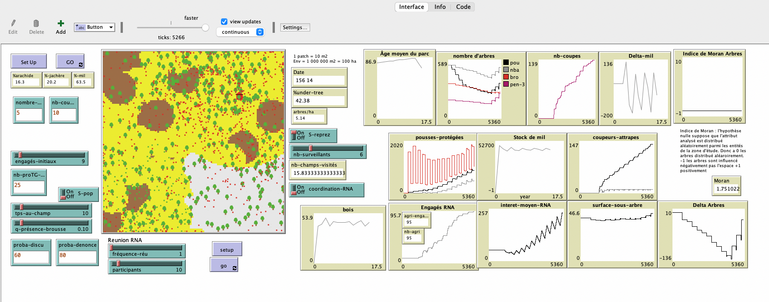
\includegraphics[height = 6cm]{img/ideModele.png}
        \end{figure}
    \end{center}
\end{frame}

\begin{frame}{Model as a plateform for ideas }
    \begin{center}
        \vspace{-1em}

        \begin{itemize}
            \item raises non-intuitive questions,
            \item feeds a global vision of the subject (Actor Network Theory)
        \end{itemize}
        \begin{figure}
            \centering
            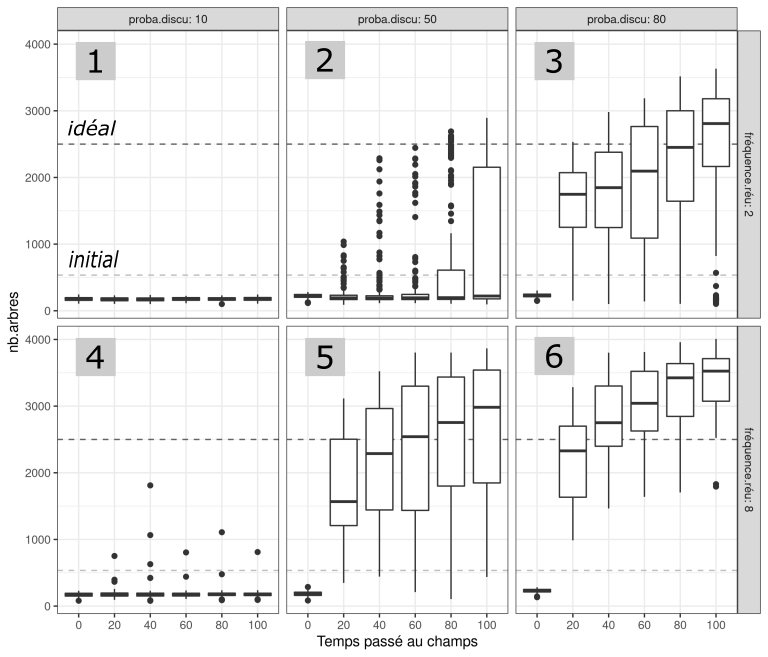
\includegraphics[height = 5.5cm]{img/boxplotReunionDiscussion.png}~
            
\includegraphics[height = 2cm]{img/OpenMOLE-Banner.png}
        \end{figure}
    \end{center}
\end{frame}

\begin{frame}{Questioning viability !}
    \begin{figure}
        \centering
        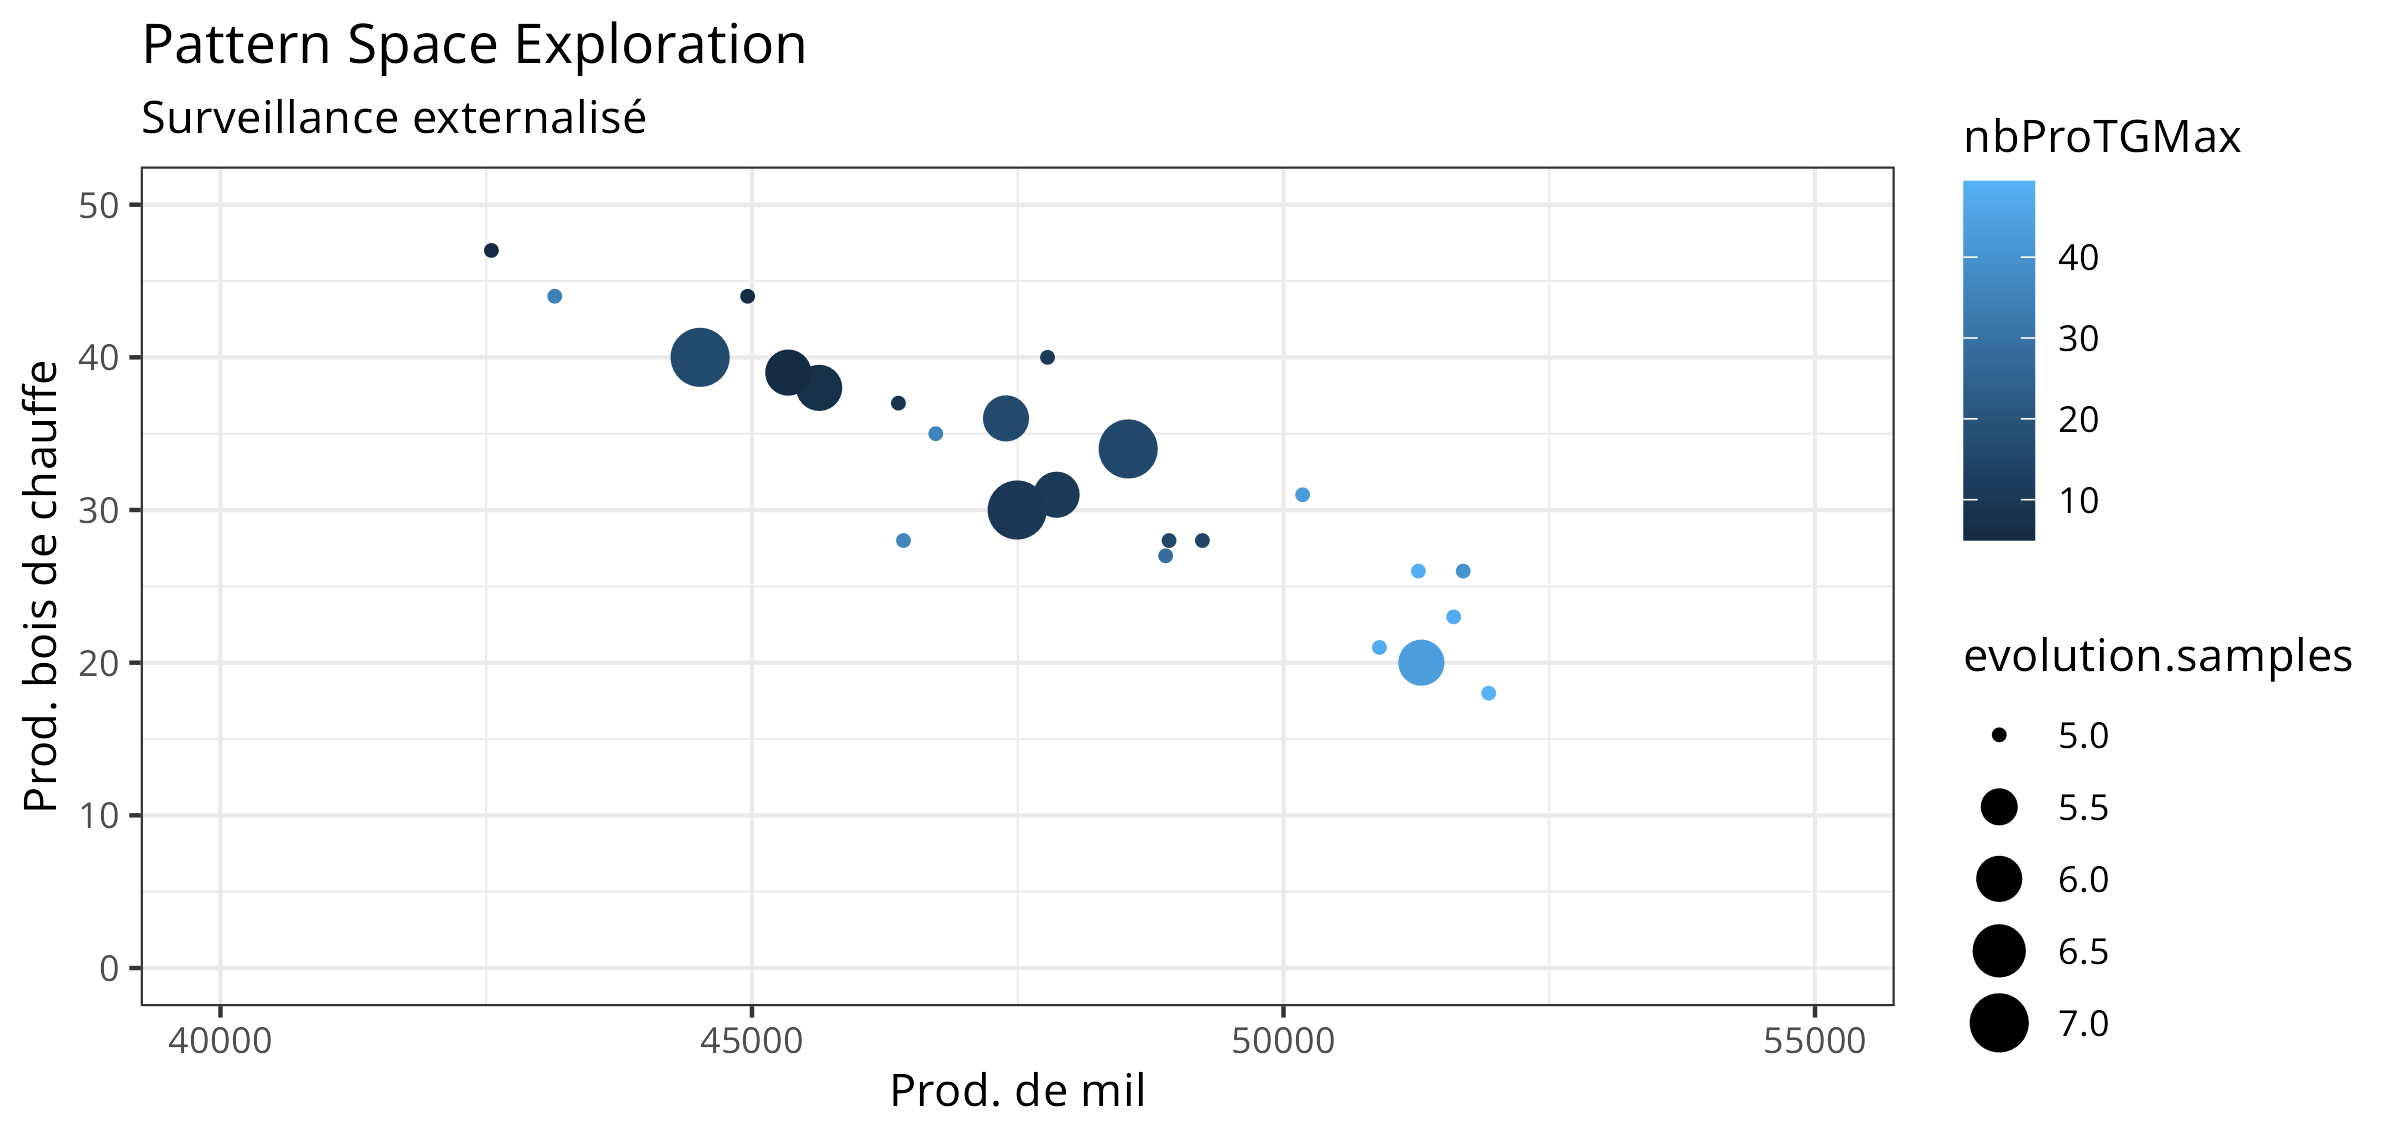
\includegraphics[height = 3.5cm]{img/om_pse_sReprez.png}~
        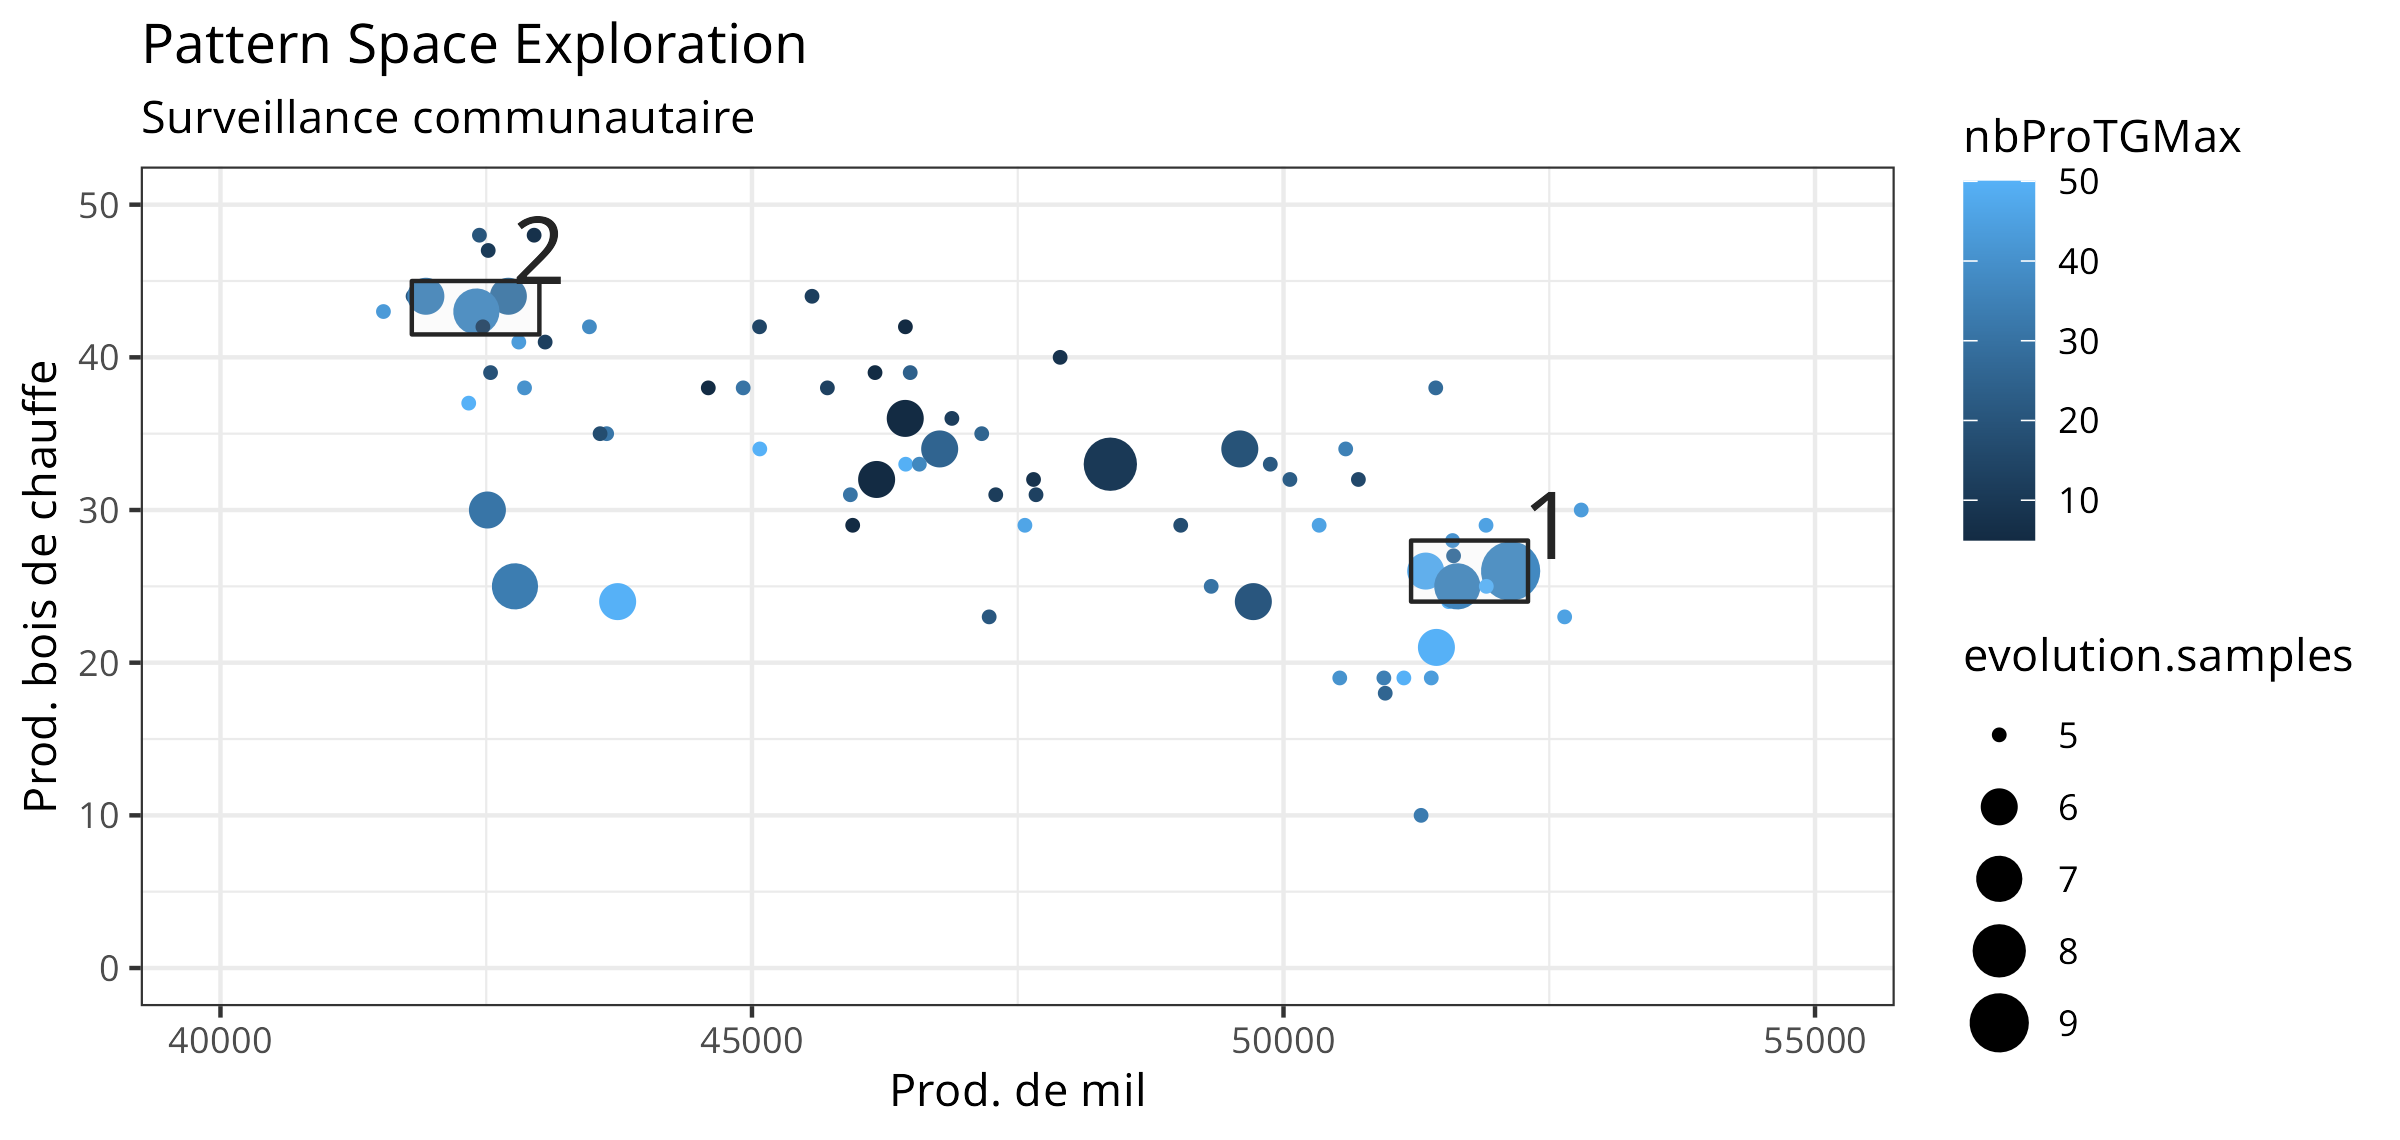
\includegraphics[height = 3.5cm]{img/om_pse_sPop.png}
    \end{figure}
\end{frame}

\begin{frame}{To conclude }
    \begin{itemize}
        \item A sight on environmental protection, revealing local tensions
        \item More a problem of tree regeneration than local monitoring
    \end{itemize}
    \begin{figure}
        \centering
        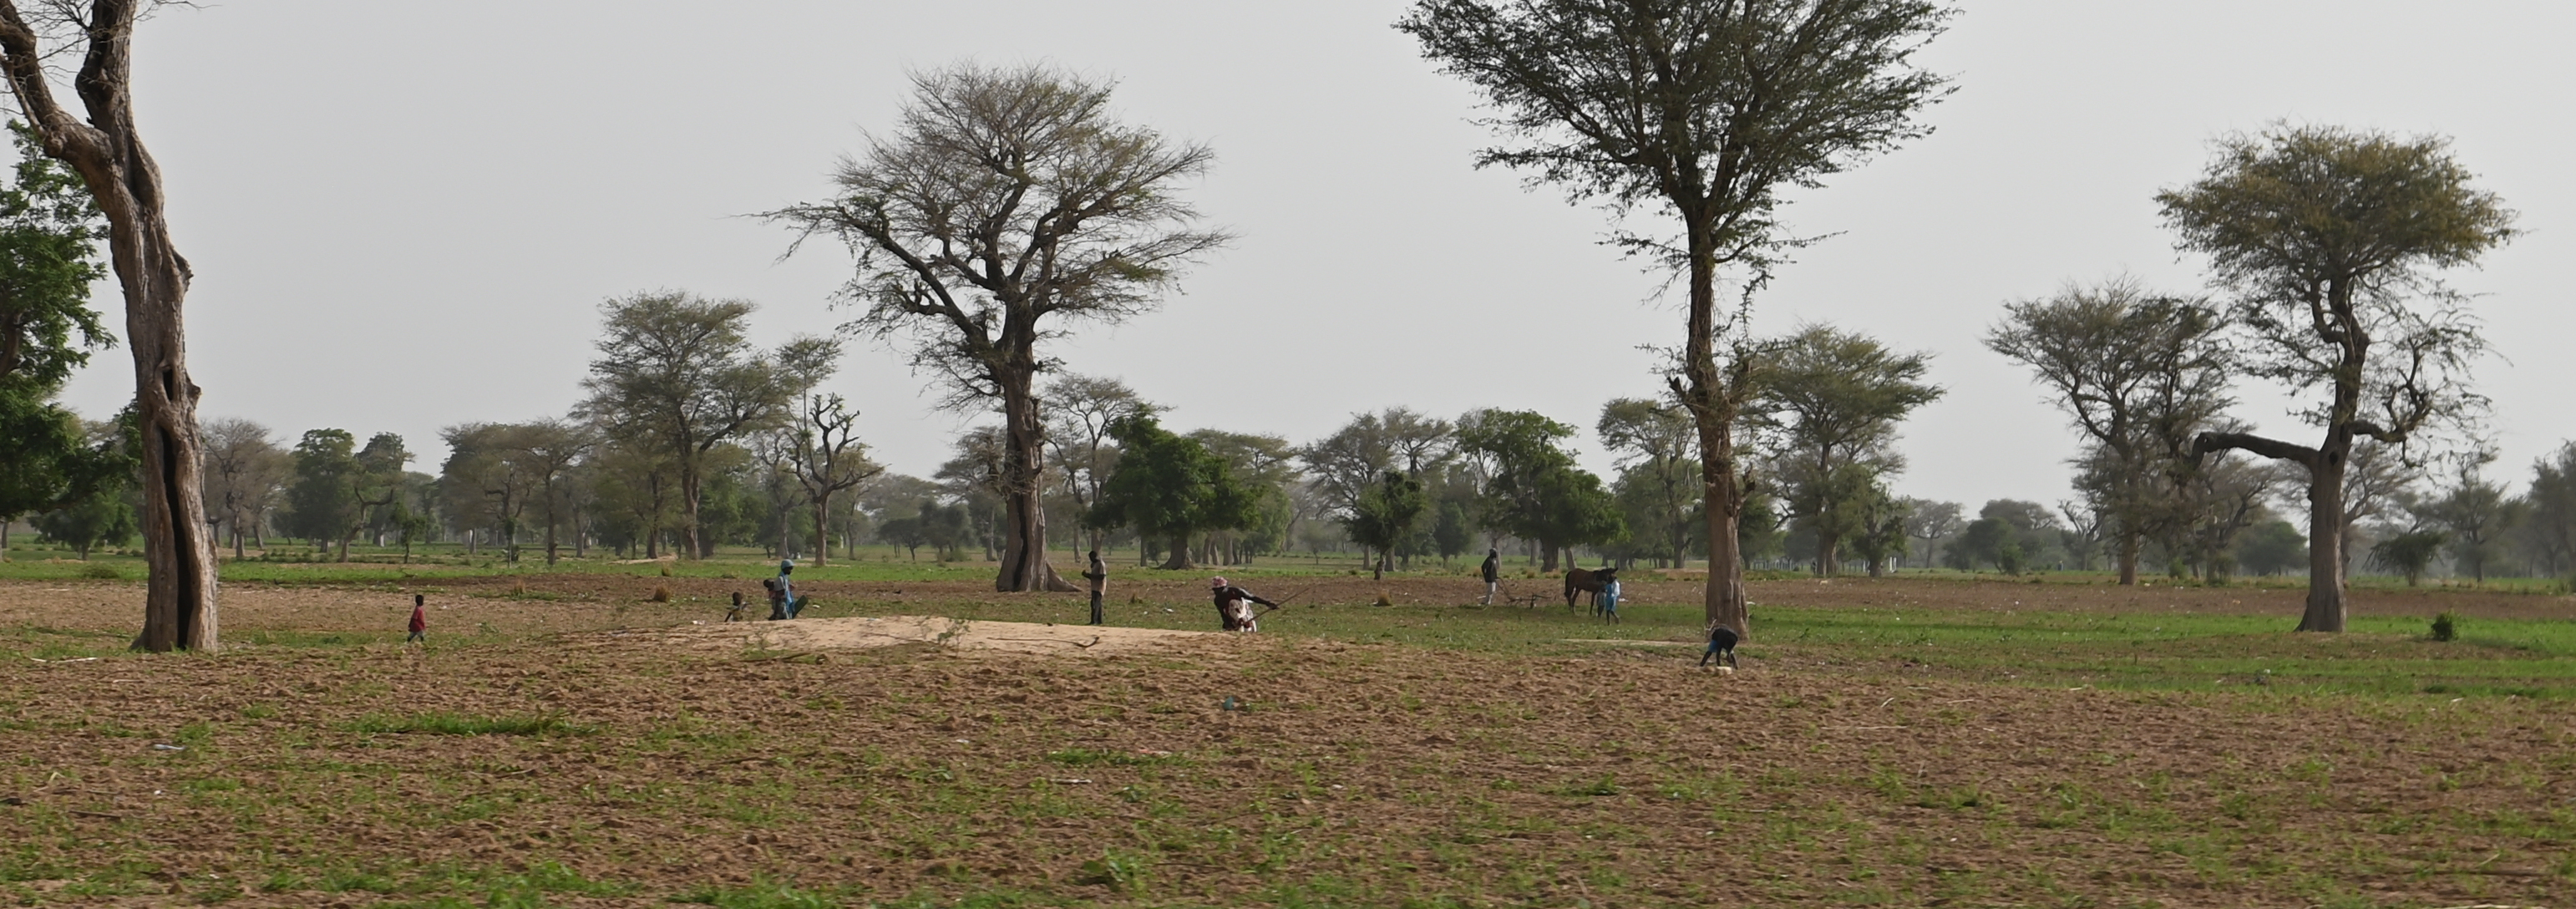
\includegraphics[height = 4cm]{img/end.JPG}
    \end{figure}
\end{frame}

\begin{frame}{Thank you for your attention !}
    \begin{figure}
        \centering
        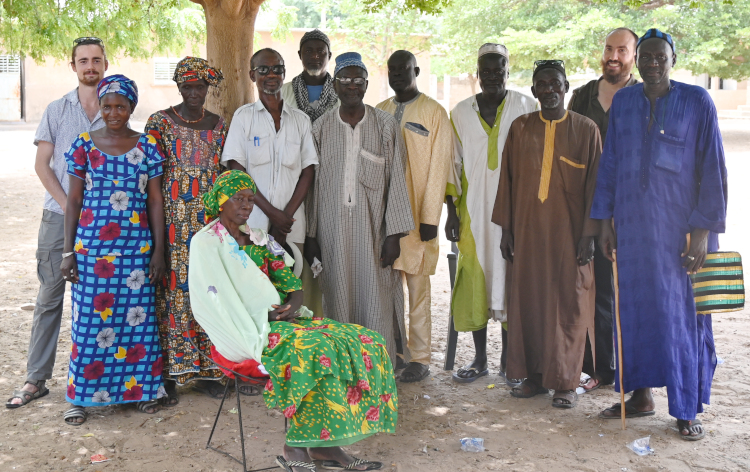
\includegraphics[height = 6cm]{img/photo_groupe.JPG}
    \end{figure}
\end{frame}

\end{document}
